% Options for packages loaded elsewhere
\PassOptionsToPackage{unicode}{hyperref}
\PassOptionsToPackage{hyphens}{url}
\PassOptionsToPackage{dvipsnames,svgnames,x11names}{xcolor}
%
\documentclass[
]{article}
\usepackage{amsmath,amssymb}
\usepackage{lmodern}
\usepackage{iftex}
\ifPDFTeX
  \usepackage[T1]{fontenc}
  \usepackage[utf8]{inputenc}
  \usepackage{textcomp} % provide euro and other symbols
\else % if luatex or xetex
  \usepackage{unicode-math}
  \defaultfontfeatures{Scale=MatchLowercase}
  \defaultfontfeatures[\rmfamily]{Ligatures=TeX,Scale=1}
  \setmainfont[]{fouriernc}
\fi
% Use upquote if available, for straight quotes in verbatim environments
\IfFileExists{upquote.sty}{\usepackage{upquote}}{}
\IfFileExists{microtype.sty}{% use microtype if available
  \usepackage[]{microtype}
  \UseMicrotypeSet[protrusion]{basicmath} % disable protrusion for tt fonts
}{}
\makeatletter
\@ifundefined{KOMAClassName}{% if non-KOMA class
  \IfFileExists{parskip.sty}{%
    \usepackage{parskip}
  }{% else
    \setlength{\parindent}{0pt}
    \setlength{\parskip}{6pt plus 2pt minus 1pt}}
}{% if KOMA class
  \KOMAoptions{parskip=half}}
\makeatother
\usepackage{xcolor}
\usepackage[margin=1in]{geometry}
\usepackage{graphicx}
\makeatletter
\def\maxwidth{\ifdim\Gin@nat@width>\linewidth\linewidth\else\Gin@nat@width\fi}
\def\maxheight{\ifdim\Gin@nat@height>\textheight\textheight\else\Gin@nat@height\fi}
\makeatother
% Scale images if necessary, so that they will not overflow the page
% margins by default, and it is still possible to overwrite the defaults
% using explicit options in \includegraphics[width, height, ...]{}
\setkeys{Gin}{width=\maxwidth,height=\maxheight,keepaspectratio}
% Set default figure placement to htbp
\makeatletter
\def\fps@figure{htbp}
\makeatother
\setlength{\emergencystretch}{3em} % prevent overfull lines
\providecommand{\tightlist}{%
  \setlength{\itemsep}{0pt}\setlength{\parskip}{0pt}}
\setcounter{secnumdepth}{-\maxdimen} % remove section numbering
\newlength{\cslhangindent}
\setlength{\cslhangindent}{1.5em}
\newlength{\csllabelwidth}
\setlength{\csllabelwidth}{3em}
\newlength{\cslentryspacingunit} % times entry-spacing
\setlength{\cslentryspacingunit}{\parskip}
\newenvironment{CSLReferences}[2] % #1 hanging-ident, #2 entry spacing
 {% don't indent paragraphs
  \setlength{\parindent}{0pt}
  % turn on hanging indent if param 1 is 1
  \ifodd #1
  \let\oldpar\par
  \def\par{\hangindent=\cslhangindent\oldpar}
  \fi
  % set entry spacing
  \setlength{\parskip}{#2\cslentryspacingunit}
 }%
 {}
\usepackage{calc}
\newcommand{\CSLBlock}[1]{#1\hfill\break}
\newcommand{\CSLLeftMargin}[1]{\parbox[t]{\csllabelwidth}{#1}}
\newcommand{\CSLRightInline}[1]{\parbox[t]{\linewidth - \csllabelwidth}{#1}\break}
\newcommand{\CSLIndent}[1]{\hspace{\cslhangindent}#1}
\newcommand{\indep}{\perp \!\!\! \perp}
\usepackage[T1]{fontenc}
\usepackage{fouriernc}
\usepackage{setspace}\onehalfspacing
\usepackage{amsfonts}
\usepackage{dcolumn}
\usepackage{pifont}
\usepackage{booktabs}
\usepackage{placeins}
\usepackage{fancyhdr}
\pagestyle{fancy}
\fancyhf{}
\rhead{Final AVCD assignment}
\lhead{1050713}
\renewcommand{\headrulewidth}{0pt}
\cfoot{\thepage}
\usepackage{booktabs}
\usepackage{longtable}
\usepackage{array}
\usepackage{multirow}
\usepackage{wrapfig}
\usepackage{float}
\usepackage{colortbl}
\usepackage{pdflscape}
\usepackage{tabu}
\usepackage{threeparttable}
\usepackage{threeparttablex}
\usepackage[normalem]{ulem}
\usepackage{makecell}
\usepackage{xcolor}
\ifLuaTeX
  \usepackage{selnolig}  % disable illegal ligatures
\fi
\IfFileExists{bookmark.sty}{\usepackage{bookmark}}{\usepackage{hyperref}}
\IfFileExists{xurl.sty}{\usepackage{xurl}}{} % add URL line breaks if available
\urlstyle{same} % disable monospaced font for URLs
\hypersetup{
  pdftitle={Economic insecurity, lack of representation and radical right voting in the context of the 2021 German federal election},
  pdfauthor={Candidate number: 1050713},
  colorlinks=true,
  linkcolor={gray},
  filecolor={Maroon},
  citecolor={Blue},
  urlcolor={magenta},
  pdfcreator={LaTeX via pandoc}}

\title{Economic insecurity, lack of representation and radical right
voting in the context of the 2021 German federal election}
\author{Candidate number: 1050713}
\date{22 May 2023}

\begin{document}
\maketitle

\hypertarget{introduction}{%
\section{Introduction}\label{introduction}}

\begin{itemize}
\item
  State research questions.
\item
  Structure of essay.
\end{itemize}

\hypertarget{motivation}{%
\section{Motivation and relation to literature}\label{motivation}}

2023 marks the tenth year of the Alternative für Deutschland's (AfD)
existence. Originally founded by a coterie of eurosceptic professors,
the AfD ran on an anti-Euro platform in the 2013 federal election
(\protect\hyperlink{ref-grimm_rise_2015}{Grimm 2015}), failing to clear
the five-percent threshold for parliamentary representation only by a
whisker.\footnote{The
  \href{https://www.bundeswahlleiterin.de/bundestagswahlen/2013/ergebnisse/bund-99.html}{AfD
  won 4.7\%} of the party votes (\emph{Zweitstimmen}).} Starting in mid
2015, as the influx of refugees rose, the AfD increasingly morphed into
a nationalistic, anti-immigration party
(\protect\hyperlink{ref-arzheimer_alternative_2017}{Arzheimer 2017};
\protect\hyperlink{ref-arzheimer_how_2019}{Arzheimer and Berning 2019};
\protect\hyperlink{ref-cantoni_persistence_2020}{Cantoni, Hagemeister,
and Westcott 2020}). With the salience of immigration high during the
2017 federal election
(\protect\hyperlink{ref-kellermann_immigration_2022}{Kellermann and
Winter 2022}), the
\href{https://www.bundeswahlleiterin.de/info/presse/mitteilungen/bundestagswahl-2017/34_17_endgueltiges_ergebnis.html}{AfD
won 12.6\%} of party votes, making it the largest opposition party. The
AfD's entry into the \emph{Bundestag} led to the debate about the
determinants of radical right support -- which had been ongoing among
political scientists at least since the late 1990s (e.g.
\protect\hyperlink{ref-kitschelt_radical_1995}{Kitschelt and McGann
1995}; \protect\hyperlink{ref-arzheimer_contextual_2009}{Arzheimer
2009}) -- gaining greater attention in both other disciplines\footnote{Guriev
  and Papaioannou (\protect\hyperlink{ref-guriev_political_2022}{2022})
  do an excellent job of summarising especially economists'
  contributions to the literature on the determinants of voting for
  populist parties.} and public discourse.

While much of the debate on the demand-side determinants of
radical-right voting has focused on the relative importance of economic
and cultural factors respectively,\footnote{Those on the economic side
  of the debate mostly do not deny the importance of cultural factors,
  such as nativist attitudes - but attribute these attitudes to economic
  factors or shocks (e.g.
  \protect\hyperlink{ref-colantone_surge_2019}{Colantone and Stanig
  2019}; \protect\hyperlink{ref-colantone_backlash_2021}{Colantone,
  Ottaviano, and Stanig 2021}). The cultural camp
  (\protect\hyperlink{ref-art_myth_2022}{Art 2022}), by contrast, sees
  such attitudes, at least in part, as exogenous to economic shocks,
  instead, conceiving of them as the key background condition without
  which economic insecurity would not have given rise to the electoral
  success of populists
  (\protect\hyperlink{ref-margalit_economic_2019}{Margalit 2019};
  \protect\hyperlink{ref-margalit_cultural_2022}{Margalit, Raviv, and
  Solodoch 2022}).} the theoretical framework I test below belongs to
another, somewhat more nascent strand of the literature. This strand
argues, inter alia, that the effect of economic grievances is likely
moderated by (i) voters' trust in political institutions, notably
parties and parliaments, and (ii) the degree to which they feel their
preferences are represented in the party system (e.g.
\protect\hyperlink{ref-dustmann_europes_2017}{Dustmann et al. 2017};
\protect\hyperlink{ref-eichengreen_populist_2018}{Eichengreen 2018};
\protect\hyperlink{ref-ivanov_economic_2023}{Ivanov 2023}). This set of
theoretical hypotheses - though often not explicitly acknowledged by
non-political-scientists - echo not only the work by Katz and Mair
(\protect\hyperlink{ref-katz_cartel_2009}{2009}) on the cartelisation of
(Western) European party systems, but also more recent work stressing
the importance of representational deficits in driving populist support
(e.g. \protect\hyperlink{ref-manow_ent-demokratisierung_2020}{Manow
2020}; \protect\hyperlink{ref-schafer_demokratische_2021}{Schäfer and
Zürn 2021}; \protect\hyperlink{ref-zurn_how_2022}{Zürn 2022};
\protect\hyperlink{ref-silva_parties_2023}{Silva and Wratil 2023}). More
importantly, these hypotheses have been subjected to little empirical
testing, with Ivanov
(\protect\hyperlink{ref-ivanov_economic_2023}{2023}) being a notable
exception, as, for instance, Sonin
(\protect\hyperlink{ref-sonin_historical_2022}{2022}) notes in his
review of the work by Eichengreen
(\protect\hyperlink{ref-eichengreen_populist_2018}{2018}). This essay is
intended as a small step towards filling this gap in the literature.

\hypertarget{theory}{%
\section{Theory and case selection}\label{theory}}

To the end, let me expatiate on the theoretical intuition outlined
above. Like many economic-insecurity-centred theories of radical right
support, the theoretical argument starts from the observation that
economic shocks, such as automation
(\protect\hyperlink{ref-boix_democratic_2019}{Boix 2019}) or trade
liberalisation (\protect\hyperlink{ref-autor_china_2013}{Autor, Dorn,
and Hanson 2013}), create winners and losers. This assumption holds true
not only for most Western European countries
(\protect\hyperlink{ref-colantone_trade_2018}{Colantone and Stanig
2018}; \protect\hyperlink{ref-milner_voting_2021}{Milner 2021}), in
general, but also for Germany, in particular
(\protect\hyperlink{ref-dauth_rise_2014}{Dauth, Findeisen, and Suedekum
2014}; \protect\hyperlink{ref-dauth_adjustment_2021}{Dauth et al.
2021}). Those losers, the argument goes on, who do not believe the
current political system can address their grievances will then turn to
populist radical right parties.

By way of unpacking this argument, note, first, that losers may believe
the political system to be incapable of redressing their economic
grievances for two distinct reasons. First, they might deem all
mainstream parties to be much of a muchness, meaning none of the
supposedly different parties is seen by losers as representing their
preferences. In that instance, losers are likely to think it does not
matter which mainstream party they vote for, or which of those parties
governs. Second, even if voters believe at least one mainstream party to
endorse policies conducive to redressing their economic grievances, they
might not trust any mainstream politician to follow through on these
promises.\footnote{This `trust' channel is distinct from a `valence'
  channel, where voters fundamentally trust politicians, but judge their
  levels of competence to differ
  (\protect\hyperlink{ref-green_politics_2017}{Green and Jennings
  2017}).}

These two reasons also show why the theory predicts economic losers to
turn to radical right parties, as opposed to left-wing parties, as a
result of their grievances. Many other economic-insecurity-type
arguments are unable to resolve this puzzle, which arises because the
latter's platforms tend to be significantly more pro-redistributive than
the former's platforms. Using the terminology by Linz
(\protect\hyperlink{ref-linz_breakdown_1978}{1978}), the reason is that
losers, as Eichengreen
(\protect\hyperlink{ref-eichengreen_populist_2018}{2018}) notes, regard
left-wing parties as loyal to the political system and in cahoots with
the other mainstream actors. So, their redistributive promises lack
credibility. By contrast, radical right parties' semi-loyalty or
disloyalty to the system means that voting for them increase the
likelihood that the political system, characterised by the mainstream
cartel (\protect\hyperlink{ref-katz_cartel_2009}{Katz and Mair 2009}),
will be disrupted.

In sum, this theoretical argument implies (at least)\footnote{Naturally,
  the argument could also be taken to imply that (i) a perceived lack of
  representation and (ii) low trust increase the probability of voting
  for the radical right. Given the space constraints and my focus on how
  these two factors moderate the effects of economic security, I
  prescind from testing these two hypotheses.} three testable
hypotheses.

\begin{itemize}
\tightlist
\item
  H1: Economic insecurity, \emph{ceteris paribus}, increases probability
  of voting for the radical right.
\item
  H2: The effect of economic insecurity on the probability of voting for
  the radical right is, \emph{ceteris paribus}, stronger for those who
  believe their interests not be represented in the current party
  system.
\item
  H3: The effect of economic insecurity is, \emph{ceteris paribus},
  stronger for those who are more distrustful of parties and/or
  parliament.
\end{itemize}

Before setting out my empirical strategy, let me briefly discuss my two
reasons for choosing the case of the 2021 German federal election.
First, the 2021 election occurred in the wake of the ``third wave'' of
the Covid-19 pandemic, which caused widespread financial insecurity
among German households, with more than one-third of households
reporting in early 2021 that they would be unable to cover unexpected
expenses of €2.000 within one month and had already started tapping into
their rainy-day funds
(\protect\hyperlink{ref-cziriak_publication_nodate}{Cziriak 2022}).
Secondly, the pandemic was, as in most other countries, a politically
contentious period, causing deep divides over the desirability and
efficacy of both non-pharmaceutical interventions, such as mask
mandates, and vaccination. The \emph{Querdenker} movement, in
particular, used their protests to stress that their interests were not
represented by any mainstream party. Both factors mean that economic
insecurity and subjectively perceived representational deficits were
likely salient in the minds of some voters, making this election a
suitable case for testing the above hypotheses.

\hypertarget{data-variables-and-operationalisation}{%
\section{Data, variables and
operationalisation}\label{data-variables-and-operationalisation}}

To test the above hypotheses, I use the \emph{German Longitudinal
Election Study's} (GLES) 2021 post-election survey\footnote{The data for
  the 2021 \emph{Nachwahlbefragung} are available
  \href{https://search.gesis.org/research_data/ZA7701}{here}.} - a
high-quality survey of a cross-section of 3424 (quasi-)randomly selected
individuals containing a rich set of questions about respondents' social
and political attitudes as well as their socio-demographic
characteristics.

\begin{itemize}
\tightlist
\item
  How do I operationalise economic insecurity?

  \begin{itemize}
  \tightlist
  \item
    unemployed (actual experience)
    (\texttt{unemp\_at\_least\_one\_year})
  \item
    fear of job loss (\texttt{job\_loss\_year\_next2yrs})
  \item
    fear of losing profession or having to change profession
    (\texttt{profession\_loss\_next2yrs})
  \item
    subjective evaluation of current economic situation
  \end{itemize}
\item
  How do I operationalise lack of representation?

  \begin{itemize}
  \tightlist
  \item
    no difference who one is voting for
  \item
    no difference who governs
  \end{itemize}
\end{itemize}

\begin{table}[!h]

\caption{\label{tab:data-summary-table}Summary of variables and their operationalisation}
\centering
\resizebox{\linewidth}{!}{
\begin{tabular}[t]{lll}
\toprule
Variable & Operationalisation & Survey item(s)\\
\midrule
\addlinespace[0.3em]
\multicolumn{3}{l}{\textbf{dependent variable}}\\
\hspace{1em}Radical right voting & dummy for AfD Zweitstimme & q114ba = 322\\
\addlinespace[0.3em]
\multicolumn{3}{l}{\textbf{independent variables}}\\
\hspace{1em}Economic insecurity & dummy for unemployment in past ten years & d17a-c\\
\hspace{1em} & fear of job loss & d18\\
\hspace{1em} & fear of losing or having to change profession & d19\\
\hspace{1em}Political system not responsive & no difference which party governs & q117\\
\hspace{1em} & no difference which party one votes for & q118\\
\hspace{1em}Trust in political system & trust in parliament & q79b\\
\hspace{1em} & trust in parties & q79c\\
\hspace{1em} & trust in politicians & q79d\\
\bottomrule
\multicolumn{3}{l}{\textsuperscript{*} Unemployment experience is, following Dauth et al (2021), defined as an individual having}\\
\multicolumn{3}{l}{been unemployed for at least one year.}\\
\multicolumn{3}{l}{\textsuperscript{*} Source: Codebook for GLES Cross-Section 2021, Post-Election, ZA7701, Dataset Version v1.0.0.}\\
\end{tabular}}
\end{table}

\begin{itemize}
\tightlist
\item
  dependent variable -\textgreater{} binary, Why?

  \begin{itemize}
  \tightlist
  \item
    Eichengreen focuses mainly on radical right, as Sonin notes
  \item
    hence focus justified
  \end{itemize}
\item
  proxy for economic insecurity -\textgreater{} justification
\end{itemize}

\hypertarget{methodology-and-results}{%
\section{Methodology and Results}\label{methodology-and-results}}

\begin{itemize}
\item
  Justify model specification.
\item
  DAG would be cool, but probably not possible.
\item
  Presentation of results + interpretation.
\item
  Caveats.

  \begin{itemize}
  \tightlist
  \item
    not causal, correlational analysis
  \end{itemize}
\end{itemize}

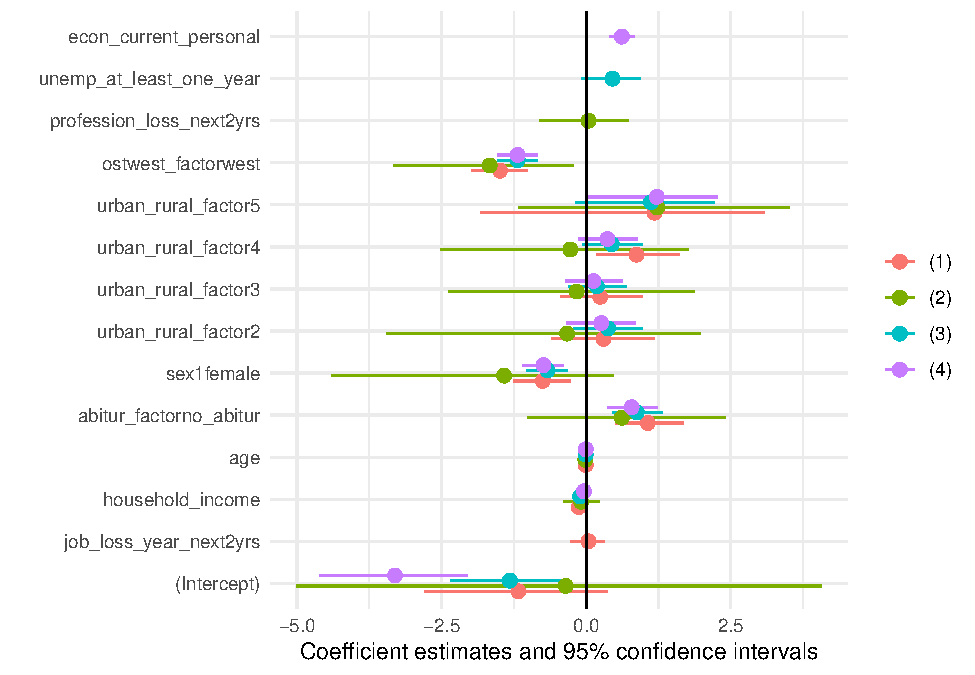
\includegraphics{AVCD_Draft_Assignment_Pruned_files/figure-latex/simple-models-insecurity-1.pdf}

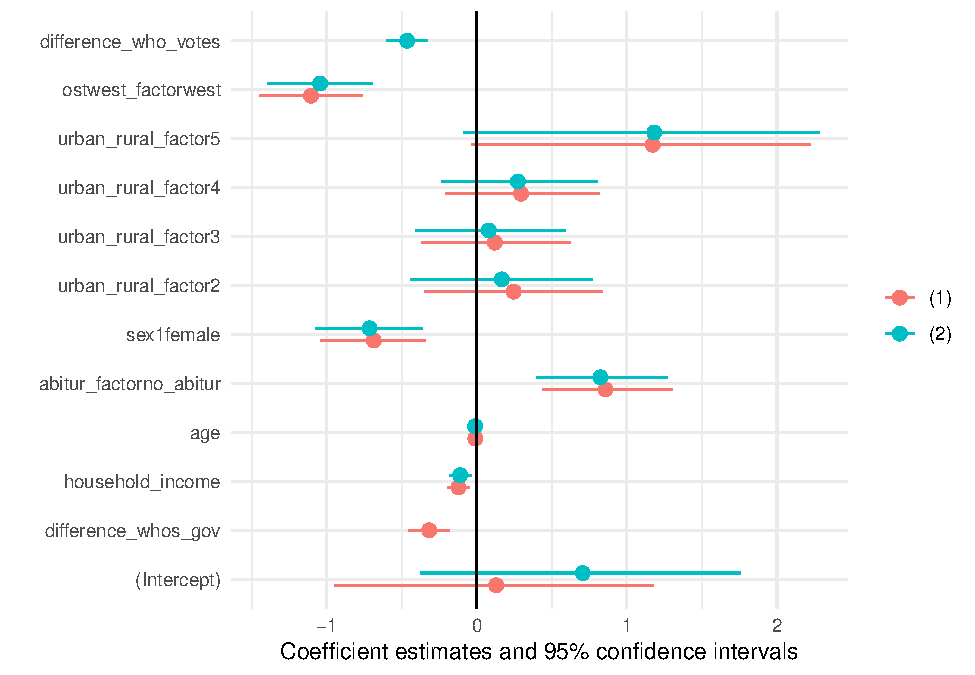
\includegraphics{AVCD_Draft_Assignment_Pruned_files/figure-latex/simple-models-lack-rep-1.pdf}

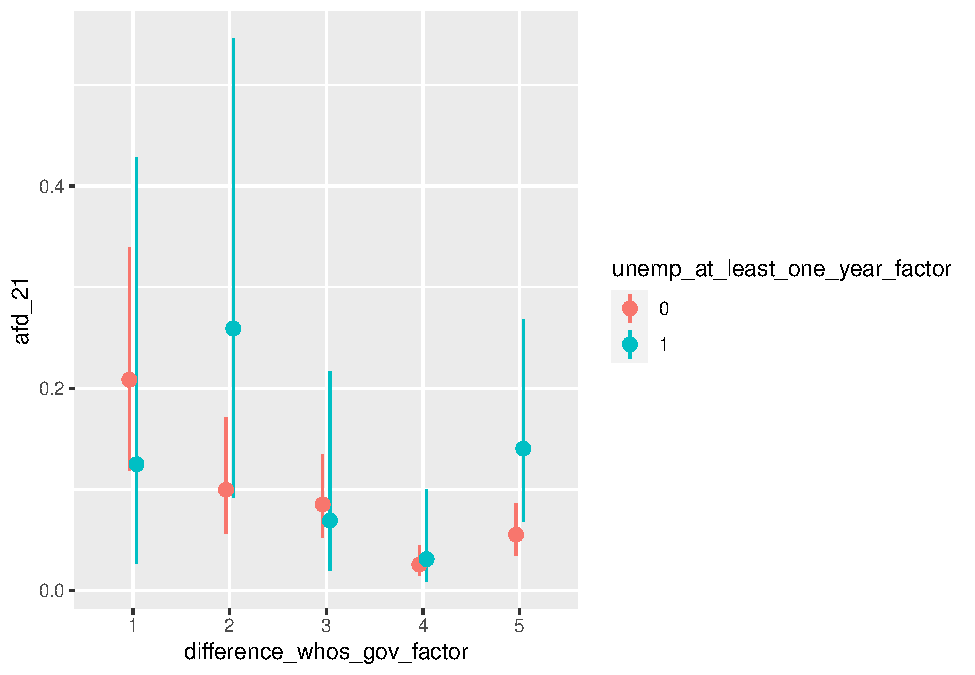
\includegraphics{AVCD_Draft_Assignment_Pruned_files/figure-latex/interaction-models-lack-rep1-1.pdf}
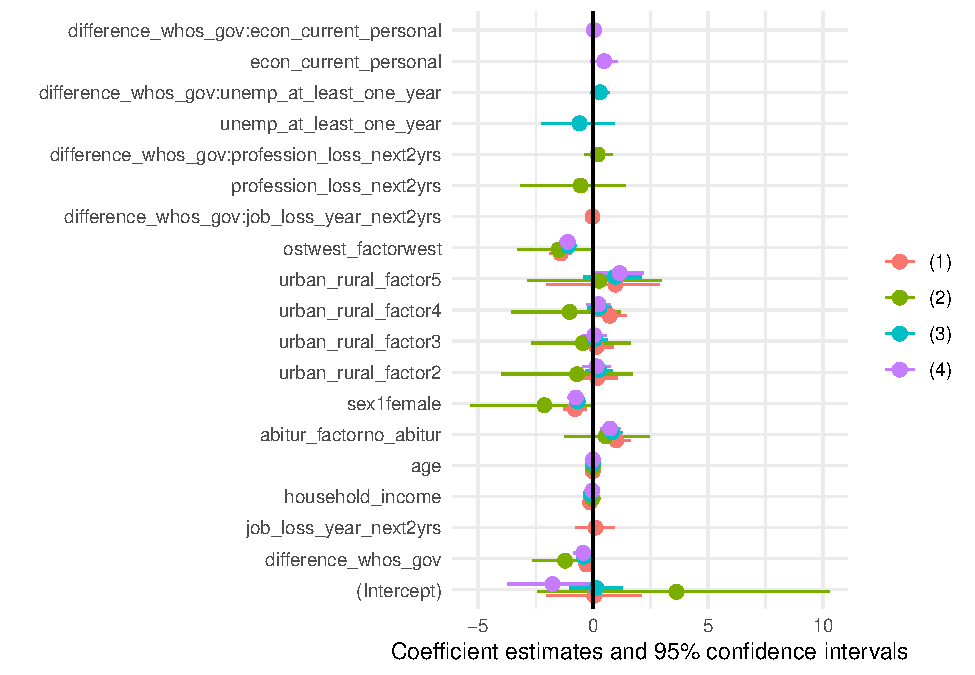
\includegraphics{AVCD_Draft_Assignment_Pruned_files/figure-latex/interaction-models-lack-rep1-2.pdf}

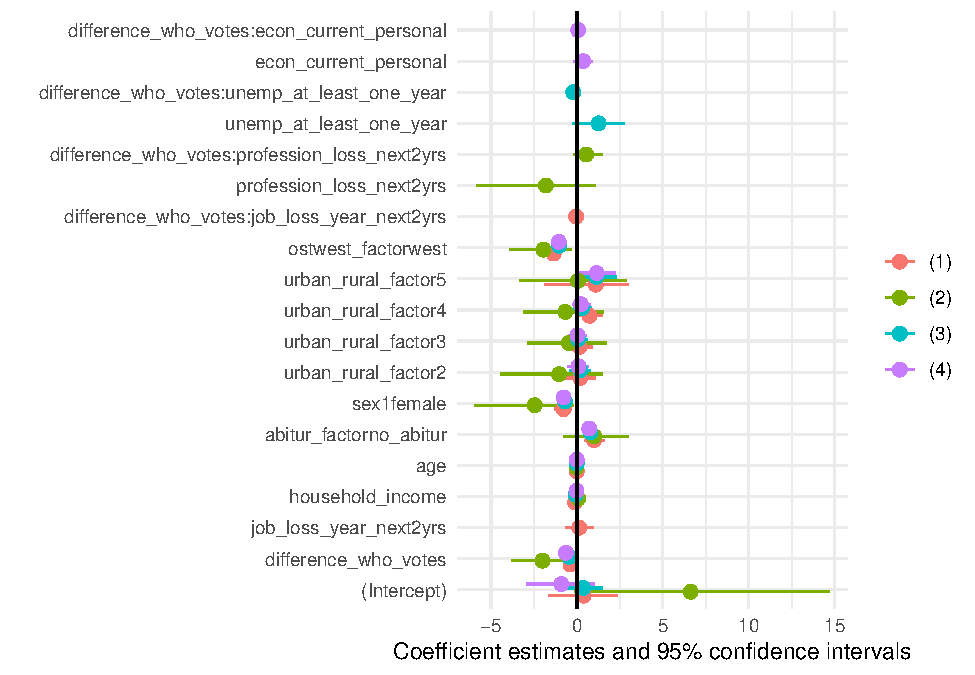
\includegraphics{AVCD_Draft_Assignment_Pruned_files/figure-latex/interaction-models-lack-rep2-1.pdf}

\hypertarget{conclusion}{%
\section{Conclusion}\label{conclusion}}

\begin{itemize}
\tightlist
\item
  I find only extremely weak support for Eichengreen's theory.
\end{itemize}

\hypertarget{references}{%
\section{References}\label{references}}

\FloatBarrier

\hypertarget{appendix}{%
\section{Appendix}\label{appendix}}

\hypertarget{descriptive-statistics}{%
\subsection{Descriptive statistics}\label{descriptive-statistics}}

\hypertarget{robustness-checks}{%
\subsection*{Robustness checks}\label{robustness-checks}}
\addcontentsline{toc}{subsection}{Robustness checks}

\hypertarget{refs}{}
\begin{CSLReferences}{1}{0}
\leavevmode\vadjust pre{\hypertarget{ref-art_myth_2022}{}}%
Art, David. 2022. {``The {Myth} of {Global} {Populism}.''}
\emph{Perspectives on Politics} 20 (3): 999--1011.

\leavevmode\vadjust pre{\hypertarget{ref-arzheimer_contextual_2009}{}}%
Arzheimer, Kai. 2009. {``Contextual {Factors} and the {Extreme} {Right}
{Vote} in {Western} {Europe}, 1980-2002.''} \emph{American Journal of
Political Science} 53 (2): 259--75.

\leavevmode\vadjust pre{\hypertarget{ref-arzheimer_alternative_2017}{}}%
---------. 2017. {``Die {Alternative} Fuer {Deutschland}.
{Programmatik}, {Entwicklung} Und Politische {Verortung}.''}
\emph{German Politics} 26 (2): 334--35.

\leavevmode\vadjust pre{\hypertarget{ref-arzheimer_how_2019}{}}%
Arzheimer, Kai, and Carl C. Berning. 2019. {``How the {Alternative} for
{Germany} ({AfD}) and Their Voters Veered to the Radical Right,
2013--2017.''} \emph{Electoral Studies} 60 (August): 102040.

\leavevmode\vadjust pre{\hypertarget{ref-autor_china_2013}{}}%
Autor, David H., David Dorn, and Gordon H. Hanson. 2013. {``The {China}
{Syndrome}: {Local} {Labor} {Market} {Effects} of {Import} {Competition}
in the {United} {States}.''} \emph{American Economic Review} 103 (6):
2121--68.

\leavevmode\vadjust pre{\hypertarget{ref-boix_democratic_2019}{}}%
Boix, Carles. 2019. \emph{Democratic {Capitalism} at the {Crossroads}:
{Technological} {Change} and the {Future} of {Politics}}. Illustrated
Edition. Princeton: Princeton Univers. Press.

\leavevmode\vadjust pre{\hypertarget{ref-cantoni_persistence_2020}{}}%
Cantoni, Davide, Felix Hagemeister, and Mark Westcott. 2020.
{``Persistence and {Activation} of {Right}-{Wing} {Political}
{Ideology}.''}
\url{http://www.davidecantoni.net/pdfs/afd_draft_20200512.pdf}.

\leavevmode\vadjust pre{\hypertarget{ref-colantone_backlash_2021}{}}%
Colantone, Italo, Gianmarco Ottaviano, and Piero Stanig. 2021. {``The
Backlash of Globalization.''} Centre for {Economic} {Performance}
{Discussion} {Paper}.
\url{https://cep.lse.ac.uk/pubs/download/dp1800.pdf}.

\leavevmode\vadjust pre{\hypertarget{ref-colantone_trade_2018}{}}%
Colantone, Italo, and Piero Stanig. 2018. {``The {Trade} {Origins} of
{Economic} {Nationalism}: {Import} {Competition} and {Voting} {Behavior}
in {Western} {Europe}.''} \emph{American Journal of Political Science}
62 (4): 936--53.

\leavevmode\vadjust pre{\hypertarget{ref-colantone_surge_2019}{}}%
---------. 2019. {``The {Surge} of {Economic} {Nationalism} in {Western}
{Europe}.''} \emph{Journal of Economic Perspectives} 33 (4): 128--51.

\leavevmode\vadjust pre{\hypertarget{ref-cziriak_publication_nodate}{}}%
Cziriak, Marius. 2022. {``Publication: {Households}' {Financial}
{Fragility} {During} the {COVID}-19 {Pandemic} in {Germany}.''} {ZEW}
{Discussion} {Paper}.
\url{https://www.zew.de/en/publications/households-financial-fragility-during-the-covid-19-pandemic-in-germany-1}.

\leavevmode\vadjust pre{\hypertarget{ref-dauth_rise_2014}{}}%
Dauth, Wolfgang, Sebastian Findeisen, and Jens Suedekum. 2014. {``The
{Rise} of the {East} and the {Far} {East}: {German} {Labor} {Markets}
and {Trade} {Integration}.''} \emph{Journal of the European Economic
Association} 12 (6): 1643--75.

\leavevmode\vadjust pre{\hypertarget{ref-dauth_adjustment_2021}{}}%
Dauth, Wolfgang, Sebastian Findeisen, Jens Suedekum, and Nicole
Woessner. 2021. {``The {Adjustment} of {Labor} {Markets} to {Robots}.''}
\emph{Journal of the European Economic Association} 19 (6): 3104--53.

\leavevmode\vadjust pre{\hypertarget{ref-dustmann_europes_2017}{}}%
Dustmann, Christian, Barry Eichengreen, Sebastian Otten, André Sapir,
Guido Tabellini, and Gylfi Zoega. 2017. {``Europe's {Trust} {Deficit}:
{Causes} and {Remedies}.''} London: Centre for Economic Policy Research.
\url{http://www.christiandustmann.com/content/4-research/14-europe-s-trust-deficit-causes-and-remedies/europe-s-trust-deficit-causes-and-remedies.pdf}.

\leavevmode\vadjust pre{\hypertarget{ref-eichengreen_populist_2018}{}}%
Eichengreen, Barry. 2018. \emph{The {Populist} {Temptation}: {Economic}
{Grievance} and {Political} {Reaction} in the {Modern} {Era}}. New York,
NY: Oxford University Press.

\leavevmode\vadjust pre{\hypertarget{ref-green_politics_2017}{}}%
Green, Jane, and Will Jennings. 2017. \emph{The {Politics} of
{Competence}: {Parties}, {Public} {Opinion} and {Voters}}. Cambridge,
UK: Cambridge University Press.

\leavevmode\vadjust pre{\hypertarget{ref-grimm_rise_2015}{}}%
Grimm, Robert. 2015. {``The Rise of the {German} {Eurosceptic} Party
{Alternative} Für {Deutschland}, Between Ordoliberal Critique and
Popular Anxiety.''} \emph{International Political Science Review} 36
(3): 264--78.

\leavevmode\vadjust pre{\hypertarget{ref-guriev_political_2022}{}}%
Guriev, Sergei, and Elias Papaioannou. 2022. {``The {Political}
{Economy} of {Populism}.''} \emph{Journal of Economic Literature} 60
(3): 753--832.

\leavevmode\vadjust pre{\hypertarget{ref-ivanov_economic_2023}{}}%
Ivanov, Denis. 2023. {``Economic {Insecurity}, {Institutional} {Trust}
and {Populist} {Voting} {Across} {Europe}.''} \emph{Comparative Economic
Studies}, February.

\leavevmode\vadjust pre{\hypertarget{ref-katz_cartel_2009}{}}%
Katz, Richard S., and Peter Mair. 2009. {``The {Cartel} {Party}
{Thesis}: {A} {Restatement}.''} \emph{Perspectives on Politics} 7 (4):
753--66.

\leavevmode\vadjust pre{\hypertarget{ref-kellermann_immigration_2022}{}}%
Kellermann, Kim Leonie, and Simon Winter. 2022. {``Immigration and
Anti-Immigrant Voting in the 2017 {German} Parliamentary Election.''}
\emph{German Economic Review} 23 (3): 341--401.

\leavevmode\vadjust pre{\hypertarget{ref-kitschelt_radical_1995}{}}%
Kitschelt, Herbert, and Anthony J. McGann. 1995. \emph{The {Radical}
{Right} in {Western} {Europe}: {A} {Comparative} {Analysis}}. Michigan:
University of Michigan Press.

\leavevmode\vadjust pre{\hypertarget{ref-linz_breakdown_1978}{}}%
Linz, Juan J. 1978. \emph{The {Breakdown} of {Democratic} {Regimes}:
{Crisis}, {Breakdown} and {Reequilibration}. {An} {Introduction}}.
Baltimore: Johns Hopkins University Press.

\leavevmode\vadjust pre{\hypertarget{ref-manow_ent-demokratisierung_2020}{}}%
Manow, Philip. 2020. \emph{({Ent}-){Demokratisierung} Der {Demokratie}}.
Berlin: Suhrkamp Verlag.

\leavevmode\vadjust pre{\hypertarget{ref-margalit_economic_2019}{}}%
Margalit, Yotam. 2019. {``Economic {Insecurity} and the {Causes} of
{Populism}, {Reconsidered}.''} \emph{The Journal of Economic
Perspectives} 33 (4): 152--70.

\leavevmode\vadjust pre{\hypertarget{ref-margalit_cultural_2022}{}}%
Margalit, Yotam, Shir Raviv, and Omer Solodoch. 2022. {``The {Cultural}
{Origins} of {Populism}.''} \{SSRN\} \{Scholarly\} \{Paper\}. Rochester,
NY. \url{https://doi.org/10.2139/ssrn.4001543}.

\leavevmode\vadjust pre{\hypertarget{ref-milner_voting_2021}{}}%
Milner, Helen V. 2021. {``Voting for {Populism} in {Europe}:
{Globalization}, {Technological} {Change}, and the {Extreme} {Right}.''}
\emph{Comparative Political Studies} 54 (13): 2286--2320.

\leavevmode\vadjust pre{\hypertarget{ref-schafer_demokratische_2021}{}}%
Schäfer, Armin, and Michael Zürn. 2021. \emph{Die Demokratische
{Regression}}. Berlin: Suhrkamp Verlag.

\leavevmode\vadjust pre{\hypertarget{ref-silva_parties_2023}{}}%
Silva, Bruno Castanho, and Christopher Wratil. 2023. {``Do Parties'
Representation Failures Affect Populist Attitudes? {Evidence} from a
Multinational Survey Experiment.''} \emph{Political Science Research and
Methods} 11 (2): 347--62.

\leavevmode\vadjust pre{\hypertarget{ref-sonin_historical_2022}{}}%
Sonin, Konstantin. 2022. {``The {Historical} {Perspective} on the
{Donald} {Trump} {Puzzle}: {A} {Review} of {Barry} {Eichengreen}'s
"{The} {Populist} {Temptation}: {Economic} {Grievance} and {Political}
{Reaction} in the {Modern} {Era}".''} \emph{Journal of Economic
Literature} 60 (3): 1029--38.

\leavevmode\vadjust pre{\hypertarget{ref-zurn_how_2022}{}}%
Zürn, Michael. 2022. {``How {Non}-{Majoritarian} {Institutions} {Make}
{Silent} {Majorities} {Vocal}: {A} {Political} {Explanation} of
{Authoritarian} {Populism}.''} \emph{Perspectives on Politics} 20 (3):
788--807.

\end{CSLReferences}

\end{document}
